% !TEX encoding = UTF-8 Unicode
\documentclass[a4paper]{article}

\usepackage{color}
\usepackage{url}
\usepackage[T2A]{fontenc} % enable Cyrillic fonts
\usepackage[utf8]{inputenc} % make weird characters work
\usepackage{graphicx}

\usepackage[english,serbian]{babel}

\usepackage[german=quotes]{csquotes}
\DeclareQuoteAlias{ngerman}{serbian}
\MakeOuterQuote{"}

\usepackage[unicode]{hyperref}
\hypersetup{colorlinks,citecolor=green,filecolor=green,linkcolor=blue,urlcolor=blue}

\usepackage{listings}

\usepackage{amsmath}

\definecolor{mygreen}{rgb}{0,0.6,0}
\definecolor{mygray}{rgb}{0.5,0.5,0.5}
\definecolor{mymauve}{rgb}{0.58,0,0.82}

\lstset{ 
  backgroundcolor=\color{white},   % choose the background color; you must add \usepackage{color} or \usepackage{xcolor}; should come as last argument
  basicstyle=\scriptsize\ttfamily,        % the size of the fonts that are used for the code
  breakatwhitespace=false,         % sets if automatic breaks should only happen at whitespace
  breaklines=true,                 % sets automatic line breaking
  captionpos=b,                    % sets the caption-position to bottom
  commentstyle=\color{mygreen},    % comment style
  deletekeywords={...},            % if you want to delete keywords from the given language
  escapeinside={\%*}{*)},          % if you want to add LaTeX within your code
  extendedchars=true,              % lets you use non-ASCII characters; for 8-bits encodings only, does not work with UTF-8
  firstnumber=1000,                % start line enumeration with line 1000
  frame=single,	                   % adds a frame around the code
  keepspaces=true,                 % keeps spaces in text, useful for keeping indentation of code (possibly needs columns=flexible)
  keywordstyle=\color{blue},       % keyword style
  language=Python,                 % the language of the code
  morekeywords={*,...},            % if you want to add more keywords to the set
  numbers=left,                    % where to put the line-numbers; possible values are (none, left, right)
  numbersep=5pt,                   % how far the line-numbers are from the code
  numberstyle=\tiny\color{mygray}, % the style that is used for the line-numbers
  rulecolor=\color{black},         % if not set, the frame-color may be changed on line-breaks within not-black text (e.g. comments (green here))
  showspaces=false,                % show spaces everywhere adding particular underscores; it overrides 'showstringspaces'
  showstringspaces=false,          % underline spaces within strings only
  showtabs=false,                  % show tabs within strings adding particular underscores
  stepnumber=2,                    % the step between two line-numbers. If it's 1, each line will be numbered
  stringstyle=\color{mymauve},     % string literal style
  tabsize=2,	                   % sets default tabsize to 2 spaces
  title=\lstname                   % show the filename of files included with \lstinputlisting; also try caption instead of title
}

\begin{document}

\title{Klasterovanje FIFA 19 igrača\\ \small{Seminarski rad u okviru kursa\\Istraživanje podataka\\ Matematički fakultet}}

\author{Jovan Dmitrović\\ jdmitrovic@gmail.com}

\date{18.~jun 2019.}

\maketitle

\abstract{
U ovom radu biće prikazana klasterovanje nad podacima iz video igre FIFA 19. Nad datim skupom podataka će biti izvršeno predprocesiranje, a zatim će biti prikazano korišćenje algoritma K-sredina, OPTICS, Kohonenovog algoritma, kao i korišćenje hijerarhijskog klasterovanja.\\ Ključne reči: \emph{klasterovanje, fudbal, istraživanje podataka}}

\tableofcontents

\newpage

\section{Uvod}
\label{sec:uvod}

Serijal FIFA video igara je jedan od najdugovečnijih serijala sportskih igara osnovan od strane američke kompanije EA Sports. Od 1993. godine pa do danas, serijal FIFA je dobijao barem jednog novog člana godišnje; sa svakom novom FIFA igrom, rastao je i broj liga i timova implementiranih u igri, da bi se u poslednjoj iteraciji, FIFA-i 19, našlo preko 700 klubova iz preko 30 liga širom sveta.

U samoj igri je prisutan i veliki broj fudbalera, pri čemu svaki od njih ima svoje karakteristike, što je velika količina podataka. Cilj ovog rada je da pokuša da klasteruje igrače i da izvede zaključke o prepoznatim klasterima.

\section{Podaci}
\label{sec:podaci}

Korišćeni podaci se mogu naći na sledećoj \href{https://www.kaggle.com/karangadiya/fifa19}{veb-strani}. U igri postoji ukupno 18207 fudbalera sa po 89 atributa. Pored meta-atributa igrača kao što su nacionalnost ili klub za koji fudbaler nastupa, među atributima se nalaze i atributi vezani za sposobnosti igrača u igri (npr. brzina, jačina šuta i slično); takvi atributi imaju opseg $[1, 99]$.

\subsection{Predprocesiranje podataka}
\label{subsec:predprocesiranje}

Iako SPSS modeler obavlja veliki deo posla automatski, neki od atributa nisu u pogodnom obliku za rad nad njima:

\begin{itemize}
  \item{\textbf{Visina} - visina je navedena vodeći se imperijalnim sistemom, navodeći stope i inče. Ovaj način zapisa je nezgodan, pa je poželjno prebaciti podatke u metrički sistem, tj. u centimetre.}
  \item{\textbf{Masa} - masa je izražena u funtama. Zarad konzistentnosti, masa je prevedena u kilograme.}
  \item{\textbf{Vrednost igrača, plata i otkupna klauzula} - finansijski podaci su izraženi pomoću skraćenica, te su oni prevedeni u konkretne cele brojeve.}
  \item{\textbf{Ocene igrača po pozicijama} - podaci su uneti u obliku zbira $x+y$, pa su ti podaci sabrani.}
\end{itemize}

Postoje i neki nominalni atributi koji neće biti uzeti u obzir kao što su: fotografija fudbalera, identifikacioni broj, zastava...

\subsubsection{Predprocesiranje podataka u programskom jeziku Python}

Kada je reč o primenjivanju klasterovanja u programskom jeziku \textit{Python}, pored transformacija podataka pomenutih u \ref{subsec:predprocesiranje}, neophodno je izvršiti neke tehnike predprocesiranja ručno, za razliku od programa \textit(SPSS Modeler). Ovo se u najvećoj meri odnosi na standardizaciju podataka, čiji je zadatak da sve numeričke atribute preslika u opseg $[0, 1]$. Standardizacija se u Python-u vrši uz pomoć \texttt{MinMaxScaler} funkcija iz paketa \texttt{sklearn.preprocessing}.

Kako se korišćenjem paketa \texttt{pandas} kategorički atributi ne prepoznaju automatski, neophodno ih je ručno transformisati u kategoričke podatke sa korektno označenim kategorijama. Nedostajuće vrednosti su zamenjene srednjom vrednošću atributa.

\section{Klasterovanje}

Za klasterovanje ovog skupa podataka biće upotrebljeno četiri algoritma:
\begin{itemize}
  \item{Algoritam K-sredina}
  \item{Kohonenov algoritam}
  \item{DBSCAN/OPTICS}
  \item{Algoritam hijerarhijskog klasterovanja}
\end{itemize}

Prva dva će biti sprovedeno uz pomoć programa \textit{IBM SPSS Modeler}, dok će druga dva biti implementirana u programskom jeziku \textit{Python}. Za ocenjivanje kvaliteta klasterovanja biće korišćen \textbf{senka koeficijent} (engl. \textit{Silhouette coefficient}), koji se računa, za svaku instancu $i$ na sledeći način:

$$ s_i = \frac{b-a}{max(a, b)} $$

U gorenavedenoj formuli $a$ je prosečna udaljenost instance $i$ od ostalih instanci u klaseru, dok je $b$ prosečno rastojanje između instance $i$ i instanci iz najbližeg susednog klastera. Senka koeficijent se nalazi u opsegu $[-1, 1]$; što je senka koeficijent bliži $1$, to je klasterovanje gušće.

\subsection{K-sredina}
\label{subsec:ksredina}

K-sredina (engl. \textit{K-means}) je algoritam koji, na osnovu korisnički definisanog parametra $k$, nalazi $k$ klastera i centre tih klastera. To znači da se taj parametar mora odabrati na neki način; iako postoje bolje metode za determinisanje najboljeg parametra, jednostavnosti radi će biti uzete sve vrednosti parametra od 2 do 5.

\begin{table}[h!]
\begin{center}
\caption{Algoritam K-sredina za različite vrednosti $k$}
\begin{tabular}{|c|c|} \hline
$k$ & Senka koeficijent\\ \hline
2 & 0.6\\
3 & 0.4\\
4 & 0.4\\
5 & 0.3\\ \hline
\end{tabular}
\label{tab:tabela1}
\end{center}
\end{table}

Iz priloženog eksperimenta, može se uočiti da algoritam K-sredina najbolje funkcioniše za $ k = 2 $. Ako se pogledaju dobijeni klasteri, postaje jasno da je ovaj metod odvojio golmane i ostale igrače. Naime, svi igrači imaju atribute koje karakterišu branjenje (kao što su npr. refleksi), ali igrači čija je prirodna pozicija na golu imaju mnogo bolje odgovarajuće atribute. Slično važi i u suprotnom slučaju, golmani nemaju dobre atribute van onih vezanih za branjenje.

Interesantniji slučajevi su kada je $ k = 3 $ ili $ k = 4 $. Kada postoje 3 klastera, igrači se dele na golmane, ofanzivne i defanzivne igrače. Na slici \ref{fig:3means_attributes} su prikazani atributi koji prikazuju razlike između klastera ofanzivnih i defanzivnih igrača:

\begin{figure}[h!]
\begin{center}
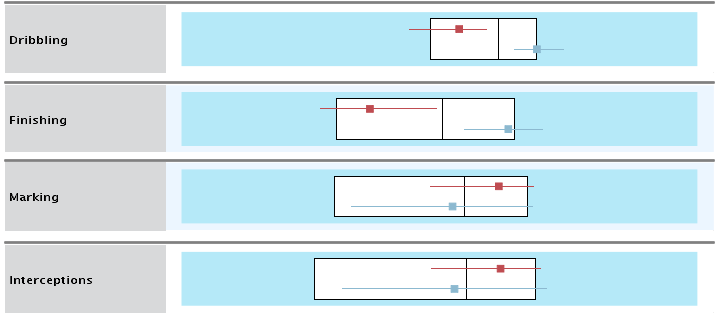
\includegraphics[width=\textwidth]{images/3means_attributes.png}
\end{center}
\caption{Neki od korišćenih atributa za algoritam 3-sredina}
\label{fig:3means_attributes}
\end{figure}

Vidimo da plavi klaster ima igrače koji su (u proseku) bolji u driblanju i realizaciji, dok crveni klaster se odlikuje boljim ocenama atributa vezanih za defanzivne zadatke, kao što su markiranje i "presecanje" dodavanja. Međutim, podela nije savršena; recimo, bekovi se ne smatraju defanzivcima jer oni često imaju i ofanzivne zadatke.

Ako se uzme da je $ k = 4 $, dobijamo do podjednako zadovoljavajućeg klasterovanja, sudeći po senka koeficijentu. Ako postoje četiri klastera, očekivani rezultat bi bio da se dobiju klasične fudbalske linije: golmani, defanzivci, napadači i vezni red. Međutim, razlika između napadača i igrača veznog reda nije velika, tako da se dobiju neočekivani rezultati. Eksperimentalnim testiranjem klasterovanja gde je $ k > 4 $ dobijaju se sve lošiji rezultati.

\subsection{Kohonenov algoritam}
\label{subsec:kohonen}

Model Kohonenovog algoritma je posebna vrsta modela neuronskih mreža koja mapira atribute u dvodimenzionalni prostor i grupiše slične instance. Ovaj model nema skrivene slojeve, već samo ulazni i izlazni sloj, pri čemu su čvorovi ulaznog sloja atributi, a čvorovi izlaznog sloja su klasteri.

Korišćenjem ovog algoritma u programu \textit{SPSS Modeler} nije dao dobre rezultate, bez obzira na prosleđene \textit{width} i \textit{length} atribute. Shodno tome, ovom algoritmu neće biti posvećeno mnogo pažnje.

\subsection{DBSCAN/OPTICS}
\label{subsec:dbscan}

DBSCAN (\textbf{D}ensity-\textbf{B}ased \textbf{S}patial \textbf{C}lustering of \textbf{A}pplications with \textbf{N}oise) je algoritam klasterovanja zasnovan na gustini. Ovaj algoritam se ponaša dobro za klastere nepravilnih oblika i za elemente van granica. 

U 2011. godini pojavio se i OPTICS algoritam\cite{optics} (\textbf{O}rdering \textbf{P}oints \textbf{T}o \textbf{I}dentify the \textbf{C}lustering \textbf{S}tructure). OPTICS se zasniva na istim osnovama kao i DBSCAN, ali donosi poboljšanje prilikom prepoznavanja klastera u prostorima manje gustine. U programskom jeziku \textit{Python}, korišćenje OPTICS algoritma ima još jednu prednost u odnosu na DBSCAN: nije neophodno unositi parametar $ \varepsilon $, jer će se on automatski izračunati. Korišćenje ovog algoritma se vrši uz pomoć funkcije \texttt{OPTICS} koja se nalazi u paketu \texttt{sklearn.cluster}.

Na slici \ref{fig:optics} je prikazano korišćenje algoritma OPTICS sa minimumom od 50 uzoraka. Tačke obojene žutom i zelenom bojom predstavljaju klastere, dok su plave tačke prepoznate kao šum. Korišćenjem ovog algoritma dobija se senka koeficijent od 0.370271 što je umereno dobar rezultat.

\begin{figure}[h!]
\begin{center}
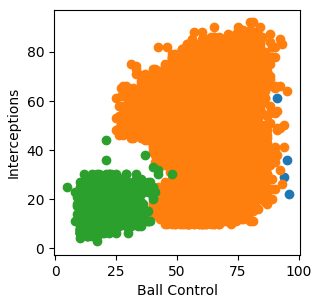
\includegraphics{images/optics.png}
\end{center}
\caption{Rezultati klasterovanja za algoritam OPTICS}
\label{fig:optics}
\end{figure}

\subsection{Hijerarhijsko klasterovanje}
\label{subsec:hijerarhijsko}

Hijerarhijsko klasterovanje izdvaja skupove ugnježdenih klastera, tako da oni formiraju hijerarhijsko stablo. Postoje dva tipa hijerarhijskog klasterovanja: \textbf{klasterovanje spajanjem} i \textbf{klasterovanje razdvajanjem}. Razlika između ova dva tipa je u početnom pristupu klasterovanju; kod spajanja, svaka instanca se posmatra kao zasebni klaster, dok se kod razdvajanja sve instance nalaze u jednom klasteru. Prilikom klasterovanja ovog skupa podataka, biće korišćeno klasterovanje spajanjem. 

Parametri neophodni za ovaj tip klasterovanja su broj klastera, mera bliskosti i kriterijum određivanja blizine klastera. Nakon korišćenja više različitih kombinacija parametara, Vardov metod\cite{ward} (engl. \textit{Ward's method}) i Euklidsko rastojanje su se pokazali najboljim. U listingu \ref{hijerarhija_py} je prikazano korišćenje ovog algoritma u programskom jeziku \textit{Python}.

\lstinputlisting[language=Python, frame=single, caption={Hijerarhijsko klasterovanje u programskom jeziku Python}, label=hijerarhija_py]{python/hijerarhija.py}

Međutim, rezultati velikim delom nisu zadovoljavajući: dobijaju se dobri rezultati isključivo za dva klastera, dok već kod tri klastera rezultati značajno opadaju. Na slici \ref{fig:ward_euclidean} su prikazani rezultati za do 5 klastera, gde su ordinati pridružene vrednosti kontrole lopte igrača, dok su apscisi pridružene vredosti presecanja lopte:

\begin{figure}[h!]
\begin{center}
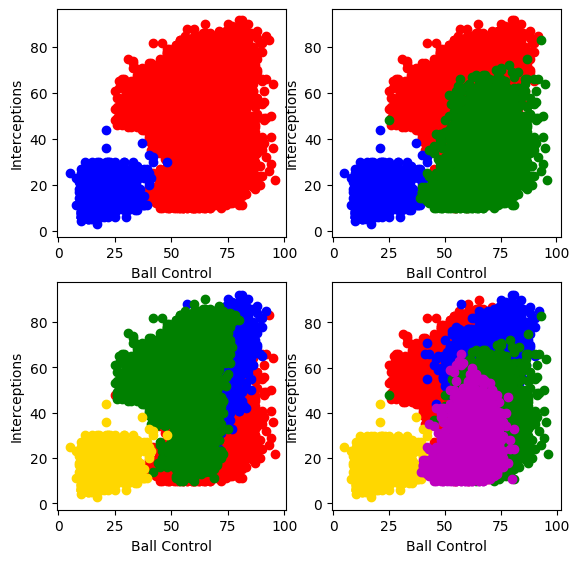
\includegraphics[width=\textwidth]{images/ward_euclidean.png}
\end{center}
\caption{Rezultati hijerarhijskog klasterovanja za 2, 3, 4 i 5 klastera}
\label{fig:ward_euclidean}
\end{figure}

Slično kao i kod algoritma K-sredina, razdvajanje igrača na golmane i "spoljne igrače" radi na zadovoljavajućem nivou. Klasterovanje sa više od dva klastera stvara probleme, tako da se senka koeficijent prepolovljava već kod tri klastera.

\section{Zaključak}
\label{sec:zakljucak}

Kod svih prikazanih metoda klasterovanja, primetno je da klasteri igrača nisu jasno izdvojivi; najčešće postoji pouzdan način da se skup podeli na 2 klastera, ali prilikom povećavanja broja klastera, dobijaju se značajno lošiji rezultati. Kao što je napomenuto u tekstu, dva klastera u pitanju su golmani i ostali igrači; postoje velike razlike u vrednostima atributa golmana i ostalih fudbalera.

Razlog loših rezultata klasterovanja je dvojak: kao prvo, fudbaleri nisu strikno vezani za pozicije i svaki igrač ima jedinstven skup sposobnosti. Takođe, neke pozicije ne pripadaju tačno jodnoj "liniji" tima (npr. bekovi, krila). Kao drugo, atributi igrača nisu eksperimentalno izmereni, niti se do njih došlo nekim naučnim putem; oni su uneti od strane razvojnog tima kompanije EA Sports, a preslikavanje sposobnosti fudbalera u numeričke atribute je možda i nemoguće.

U radu sa ovim skupom podataka, došlo se do zaključka da on nije najpogodniji za primenu klasterovanja; štaviše, stiče se utisak da bi primena klasifikacije nad ovim podacima, gde bi klase bile pozicije fudbalera, bila bolji pristup za njihovo bolje razumevanje.

\addcontentsline{toc}{section}{Literatura}
\appendix
\bibliography{seminarski} 
\bibliographystyle{plain}

\end{document}
